\chapter{Конструкторская часть}

\section{Требования к программному обеспечению}

К разрабатываемой программе предъявлен ряд требований:

\textbf{Входные данные:} Массив целых чисел, искомое целое число.

\textbf{Выходные данные:} Индекс искомого числа в массиве.

\begin{itemize}
	\item Индексация элементов в массиве начинается с 0;
	\item В случае, если искомого элемента в массиве нет, вместо индекса должно возвращаться значение -1.
\end{itemize}


\section{Вариации бинарного поиска}
Алгоритм бинарного поиска может быть описан двумя способами – итерационно и рекурсивно.

При итерационной реализации выделяют две переменные – левую и правую границы, в цикле считается средний элемент по границам и в зависимости от него эти границы меняются.

В рекурсивной реализации выбирается серединный элемент по всему массиву, и в зависимости от его значения рекурсивно вызывается поиск либо от правой части массива, либо от левой.

Для данной работы была выбрана итерационная вариация алгоритма, так как в общем случае рекурсивный вызов – трудоёмкая операция, при этом нет сложностей в реализации итерационной вариации.
\section{Разработка алгоритмов}
На рисунке \ref{fig:LS} представлена схема разработанного алгоритма линейного поиска. На рисунке \ref{fig:BS} представлена схема итерационного алгоритма бинарного поиска.


\begin{figure}[h]
	\centering
	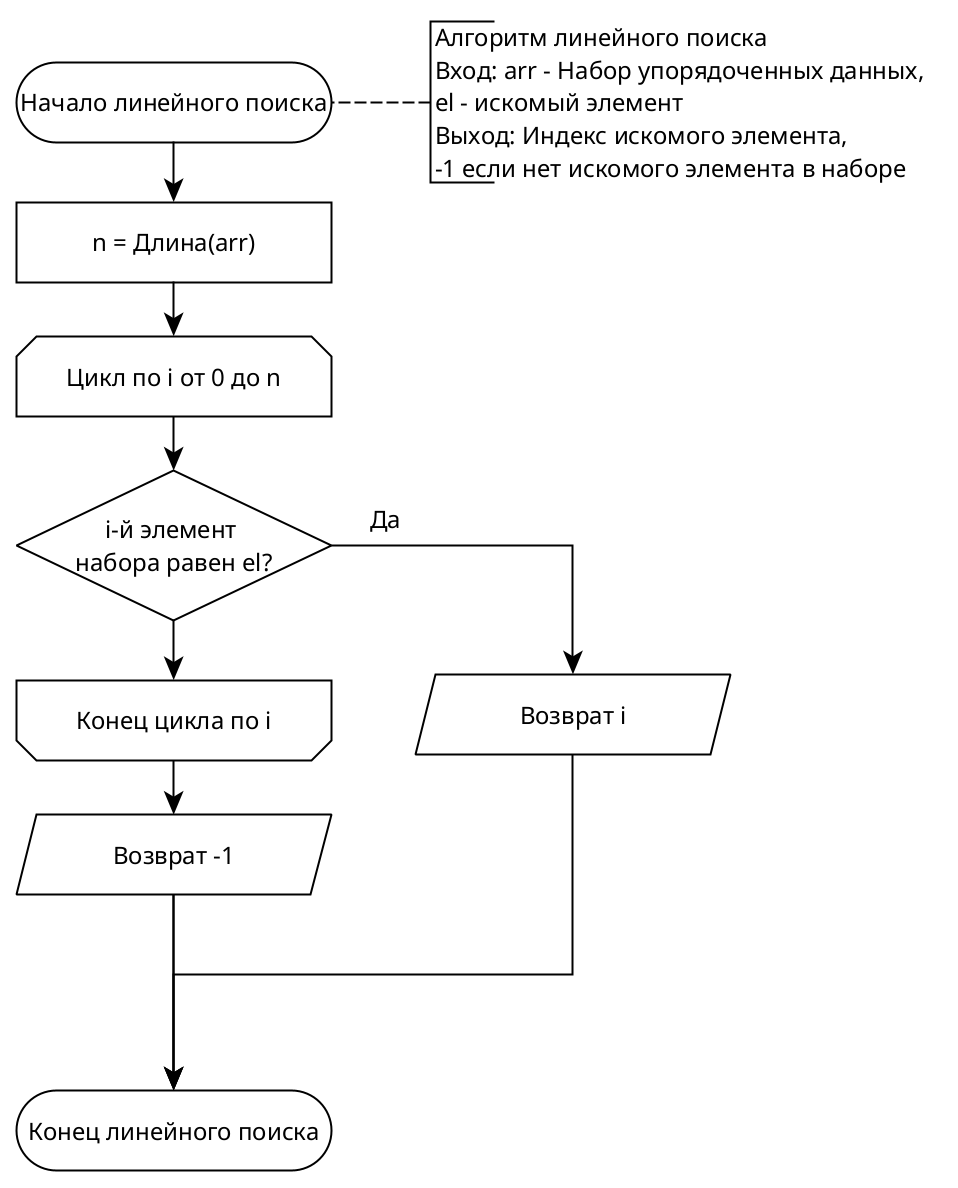
\includegraphics[width=0.9\textwidth]{LS}
	\caption{Схема алгоритма линейного поиска}
	\label{fig:LS}
\end{figure}


\begin{figure}[h]
	\centering
	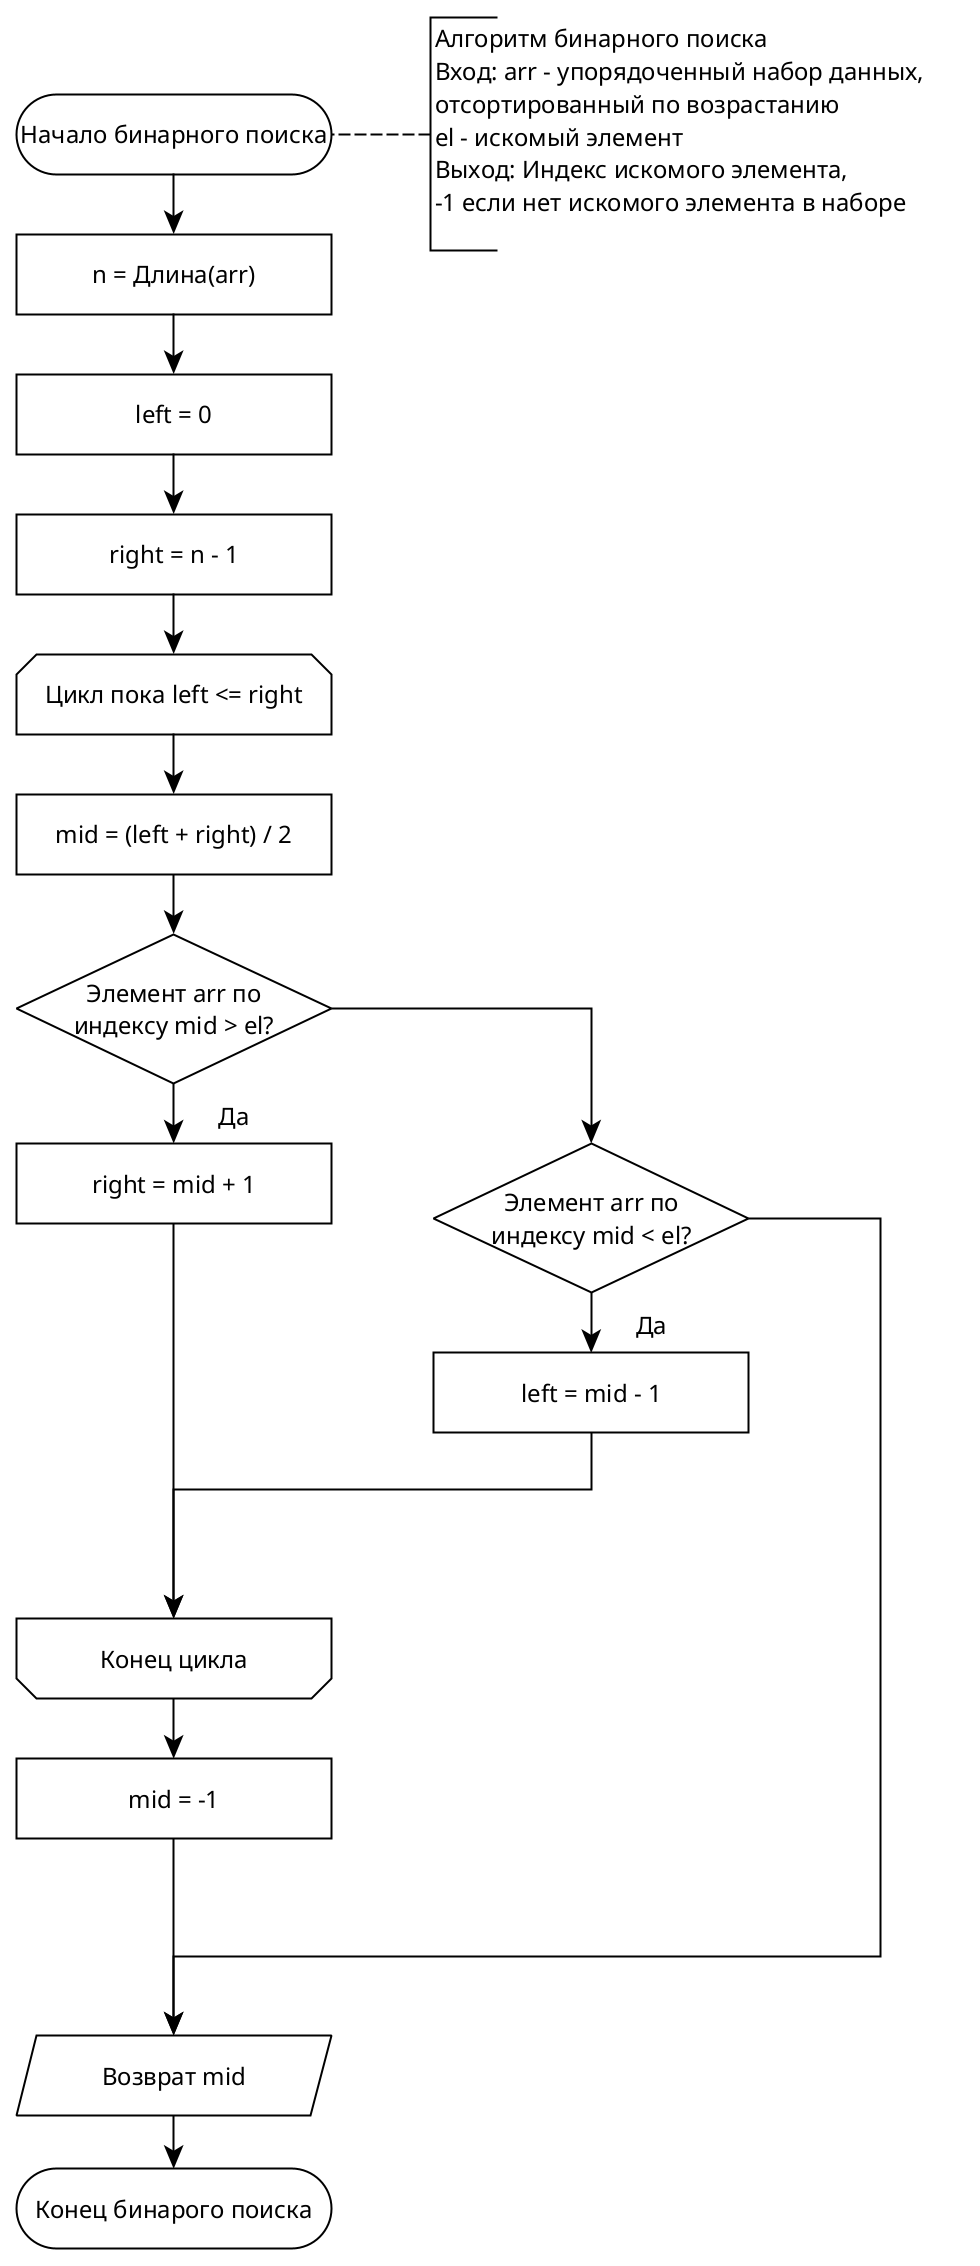
\includegraphics[width=0.9\textwidth]{BS}
	\caption{Схема алгоритма итерационного бинарного поиска}
	\label{fig:BS}
\end{figure}

\clearpage

\section{Вывод}

В результате конструкторской части были определены требования к ПО, а также разработаны схемы алгоритмов линейного поиска и бинарного поиска.

\clearpage
